\documentclass{article}
\usepackage[utf8]{inputenc}
\usepackage{authblk}
\usepackage{setspace}
\usepackage[margin=1.25in]{geometry}
\usepackage{graphicx}
\usepackage{xcolor}
\usepackage{float}
\graphicspath{ {./figures/} }
\usepackage{amsmath,amssymb,amsfonts}
\usepackage{booktabs}
\usepackage{natbib}
\usepackage{hyperref}
\hypersetup{colorlinks=true, linkcolor=blue, citecolor=blue, urlcolor=blue}

\title{\textbf{Day-of-the-Week Effects in Cryptocurrency Returns}}
\author[1]{SIQuant Research}
\affil[1]{Hypothesis $\times$ Quant}
\date{\today}
\onehalfspacing

\begin{document}
\maketitle

\begin{abstract}
\noindent \textbf{Hypothesis:} $H_0$: the mean daily return of an equal-weight crypto basket is the same on all weekdays; $H_1$: at least one weekday differs \\
\textbf{Data:} 3,272 days with at least three assets, 2017-11-10 to 2026-10-25 \\
\textbf{Method:} Weekday dummies with Newey--West HAC errors (7 lags) and a joint Wald test of the six dummies \\
\textbf{Results:} Wald $\chi^2_6=10.70$, $p=0.0983$; highest mean Sat (0.607\%), lowest Thu (0.010\%). \\
\textbf{Research decision:} \colorbox[rgb]{0.75,0.15,0.15}{\textcolor{white}{\textbf{\,REJECTED\,}}}
\end{abstract}

\section{Design}
Crypto markets trade every day, so weekday patterns can arise from the weekly rhythm of institutional and retail activity \citep{caporale2019day}. The test is a single joint hypothesis on all weekdays rather than a search for the best day, which avoids data-snooping across seven comparisons.

\section{Results}
\begin{table}[H]
\centering
\caption{Equal-weight crypto basket return by weekday (UTC)}
\begin{tabular}{lccc}
\toprule
Weekday & Days & Mean & Std. dev. \\
\midrule
Mon & 467 & 0.142\% & 4.60\% \\
Tue & 467 & 0.106\% & 4.14\% \\
Wed & 467 & 0.352\% & 4.85\% \\
Thu & 467 & 0.010\% & 5.25\% \\
Fri & 468 & 0.506\% & 4.36\% \\
Sat & 468 & 0.607\% & 3.37\% \\
Sun & 468 & 0.028\% & 3.52\% \\
\bottomrule
\end{tabular}
\end{table}


\begin{figure}[H]
\centering
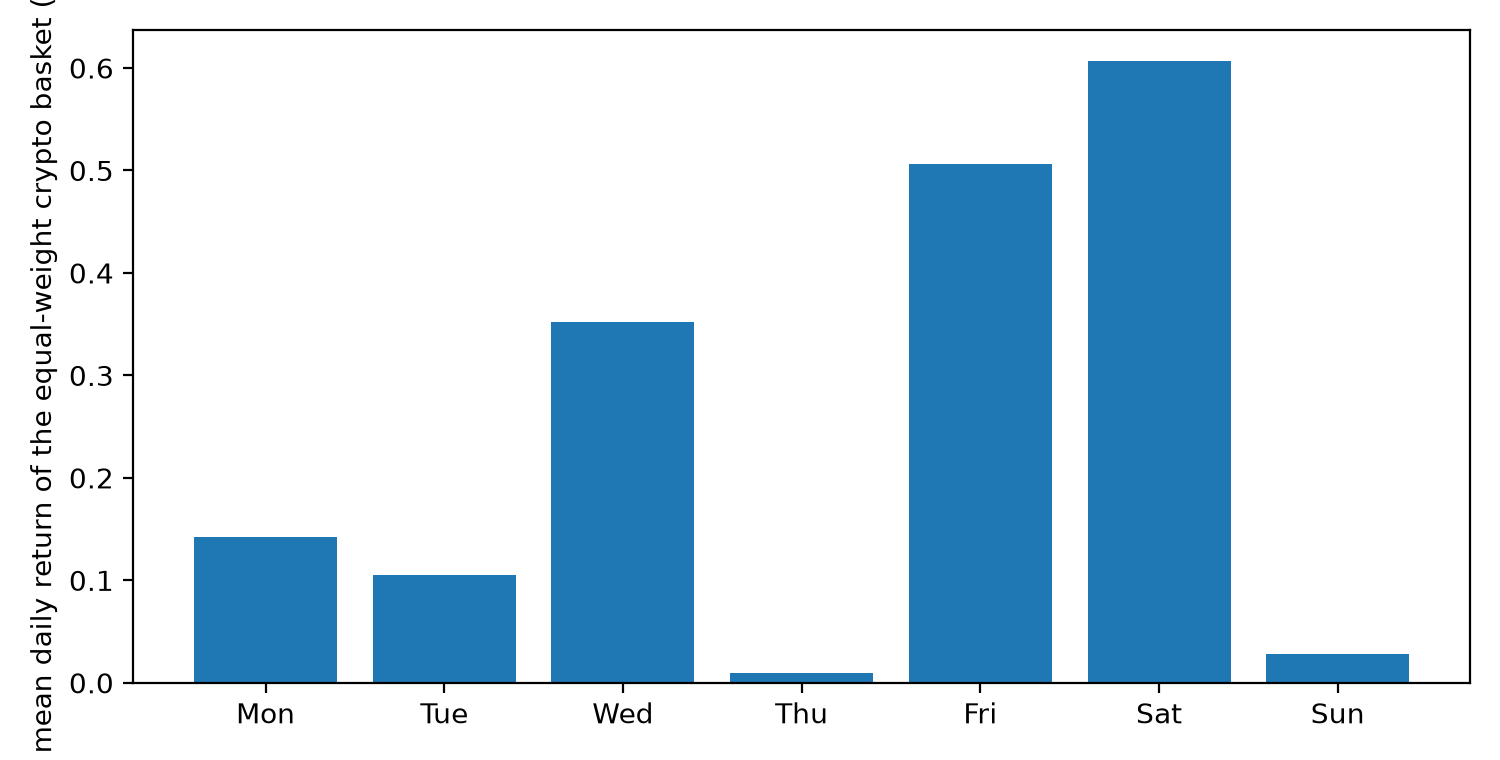
\includegraphics[width=0.8\textwidth]{fig1_crypto_day_of_week.png}
\caption{Mean daily return by weekday.}
\end{figure}

\section{Limitations}
Daily bars close at 00:00 UTC, so the weekday label follows UTC rather than any local trading day. The basket includes more assets in later years. The decade has a few extreme days, and the joint test is not robust to a single outlier driving one weekday's mean.


\bibliographystyle{plainnat}
\bibliography{references}

\end{document}
